% Gráfico editável em PGFPlots; classificação baseada nos metadados compilados.
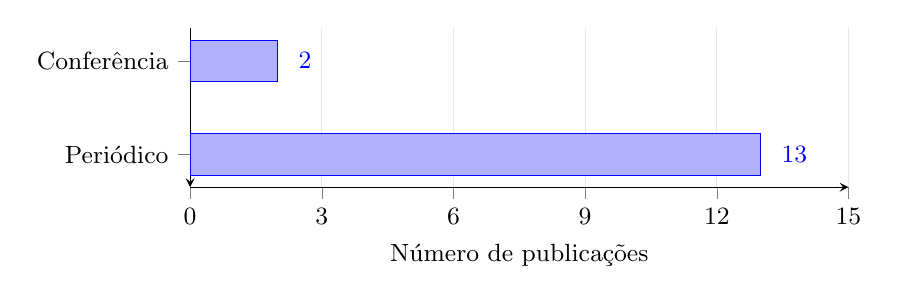
\begin{tikzpicture}
\begin{axis}[
  xbar, width=0.82\textwidth, height=3.6cm,
  xmin=0, xmax=15, xlabel={Número de publicações},
  ytick={1,2}, yticklabels={Conferência,Periódico}, y dir=reverse,
  xtick={0,3,6,9,12,15},
  axis lines=left, tick align=outside,
  xmajorgrids=true, grid style={gray!18},
  tick label style={font=\small}, label style={font=\small},
  yticklabel style={font=\small},
  nodes near coords, nodes near coords style={font=\small\bfseries, xshift=4pt},
  bar width=15pt, enlarge y limits=0.35,
  every axis plot/.append style={fill=teal!65!blue, draw=teal!65!blue!80!black}
]
\addplot coordinates {(2,1) (13,2)};
\end{axis}
\end{tikzpicture}
